%
% $RCSfile: hierarchical_model_view_controller.tex,v $
%
% Copyright (c) 2004. Christian Heller. All rights reserved.
%
% No copying, altering, distribution or any other actions concerning this
% document, except after explicit permission by the author!
% At some later point in time, this document is planned to be put under
% the GNU FDL license. For now, _everything_ is _restricted_ by the author.
%
% http://www.cybop.net
% - Cybernetics Oriented Programming -
%
% http://www.resmedicinae.org
% - Information in Medicine -
%
% @author Christian Heller <christian.heller@tuxtax.de>
%

\paragraph{Hierarchical Model View Controller}
\label{hierarchical_model_view_controller_heading}

There exist several extensions of the MVC pattern, one of them being the
\emph{Hierarchical Model View Controller} (HMVC) \cite{cai}. It combines the
patterns \emph{Composite}, \emph{Layers} and \emph{Chain of Responsibility}
into one conceptual architecture (figure \ref{hmvc_figure}).

This architecture divides the presentation layer into hierarchical sections
containing so-called \emph{MVC Triads}. The triads conventionally consist of
\emph{Model}, \emph{View} and \emph{Controller}, each. They communicate with
each other by relating over their controller object. Following the \emph{Layers}
pattern, only neighbouring layers know from each other.

As a practical example, the upper-most triad could represent a graphical
\emph{Dialog} and the next lower one a \emph{Panel}. Being a container, too,
the panel could hold a third triad like for example a \emph{Button}. Events
occuring at the button are then normally processed by the corresponding
controller belonging to the button's triad. If, however, the button controller
cannot handle the event, that is forwarded along the chain of responsibility to
the controller of the higher-next layer. If also the panel controller does not
know how to handle the event, the final responsibility falls to the controller
of the dialog's triad.

The HMVC is similar to the \emph{Presentation Abstraction Control} (PAC) pattern
\cite{buschmann}. A \emph{PAC Agent} is comparable to an \emph{HMVC Triad}.

\begin{figure}[ht]
    \begin{center}
        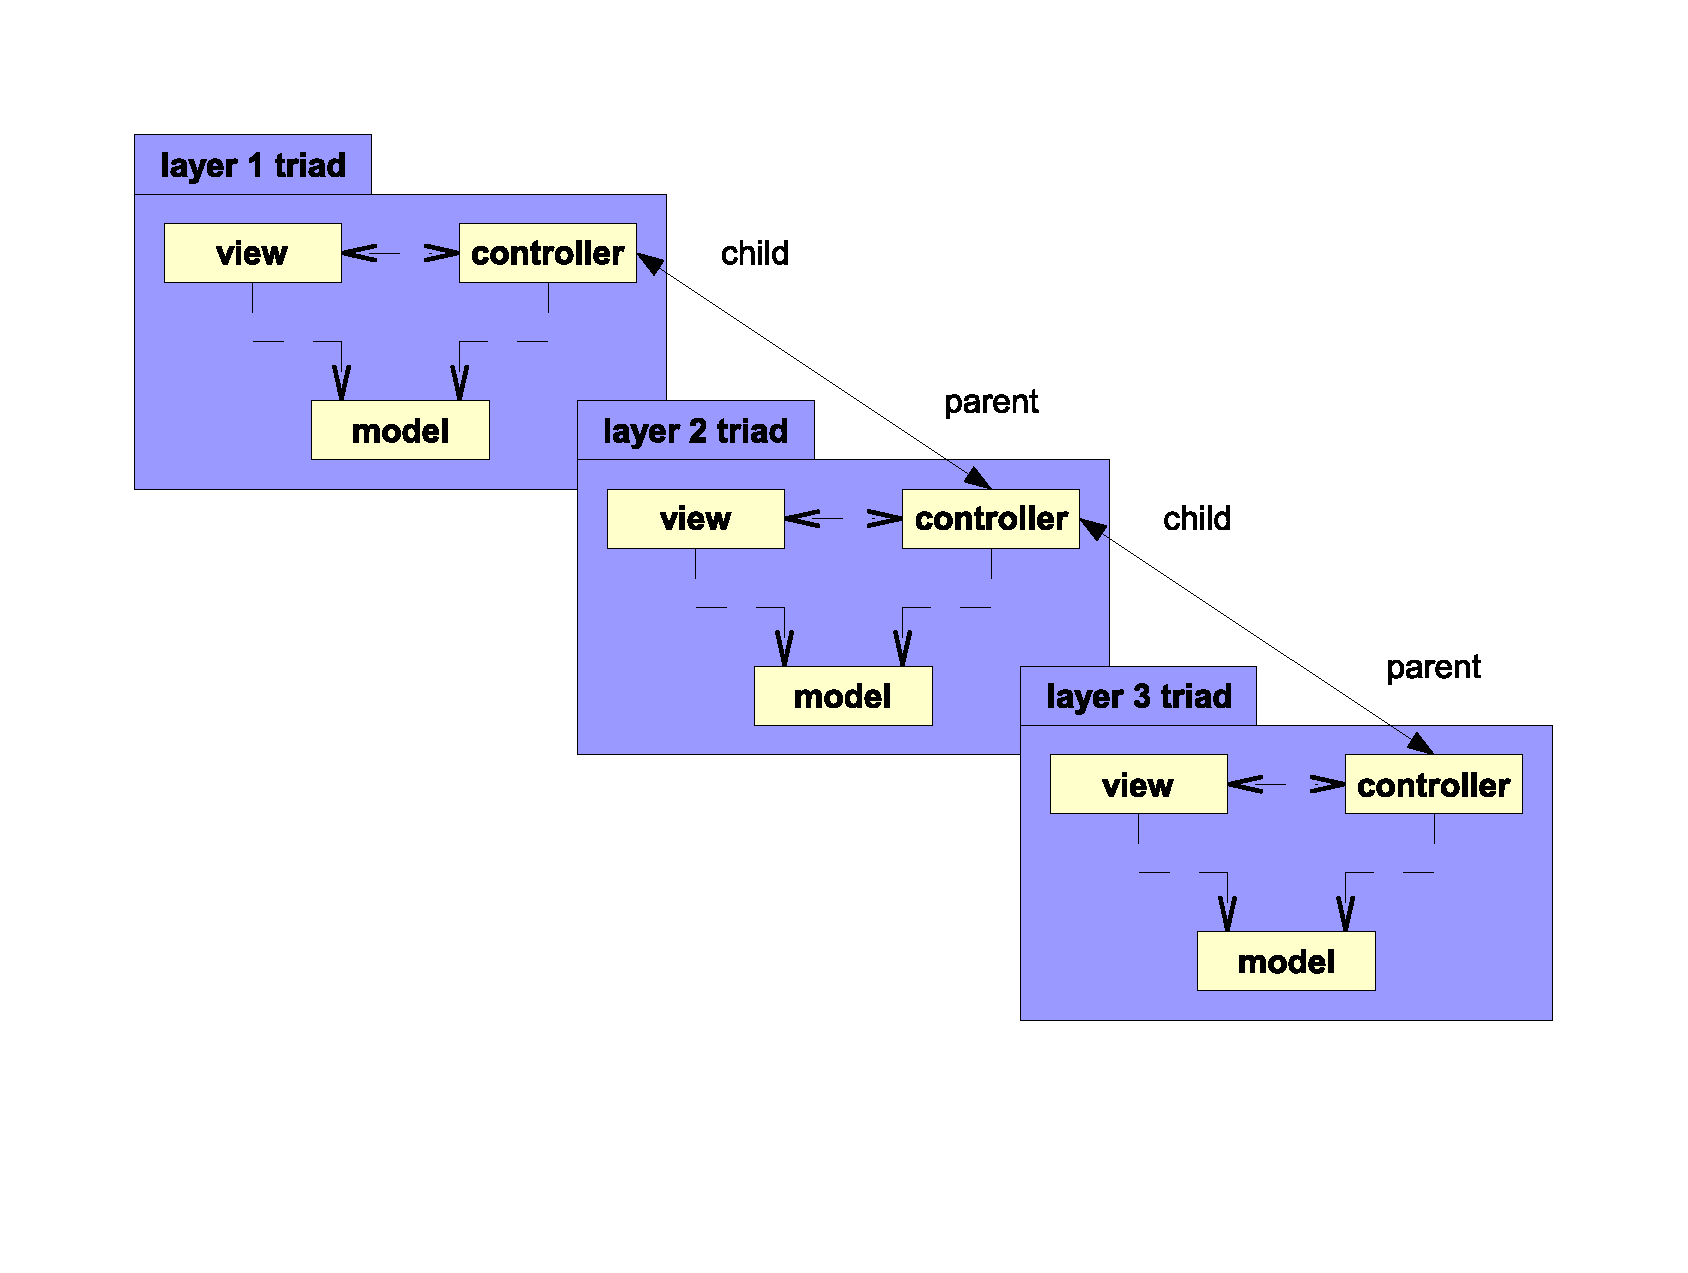
\includegraphics[scale=0.3]{vector/hmvc.eps}
        \caption{Hierarchical Model View Controller Pattern}
        \label{hmvc_figure}
    \end{center}
\end{figure}
